\chapter{Conclusions}
\label{chapter:conclusions}

This thesis examined different technical solutions to managing, sharing and
publishing research data, focusing on sharing and publishing. Table
\ref{fig:solutions} shows the different technical solutions and how they
differ in terms of features in the context of research data publishing.

TODO: add here explanations on what the different columns mean

Notable in the table is that the existing solutions to research data publishing
do not take into account the long term storage of research data. The one
solution that does that, PAS, only focuses on that making it imperative that
the systems that are used to publish the research data should be integrated to
a system that provides long term archival as well. The open source tools offer
a notably similar set of features and any one of them could be taken into use
and it would serve as a serviceable technical platform for research data
publishing.

The identifier scheme is also a point of interest. Citing datasets is something
that has not been widely adopted, which means that in order to help that
adoption a well known identifier scheme should be used.

\begin{sidewaysfigure}
    \begin{centering}
        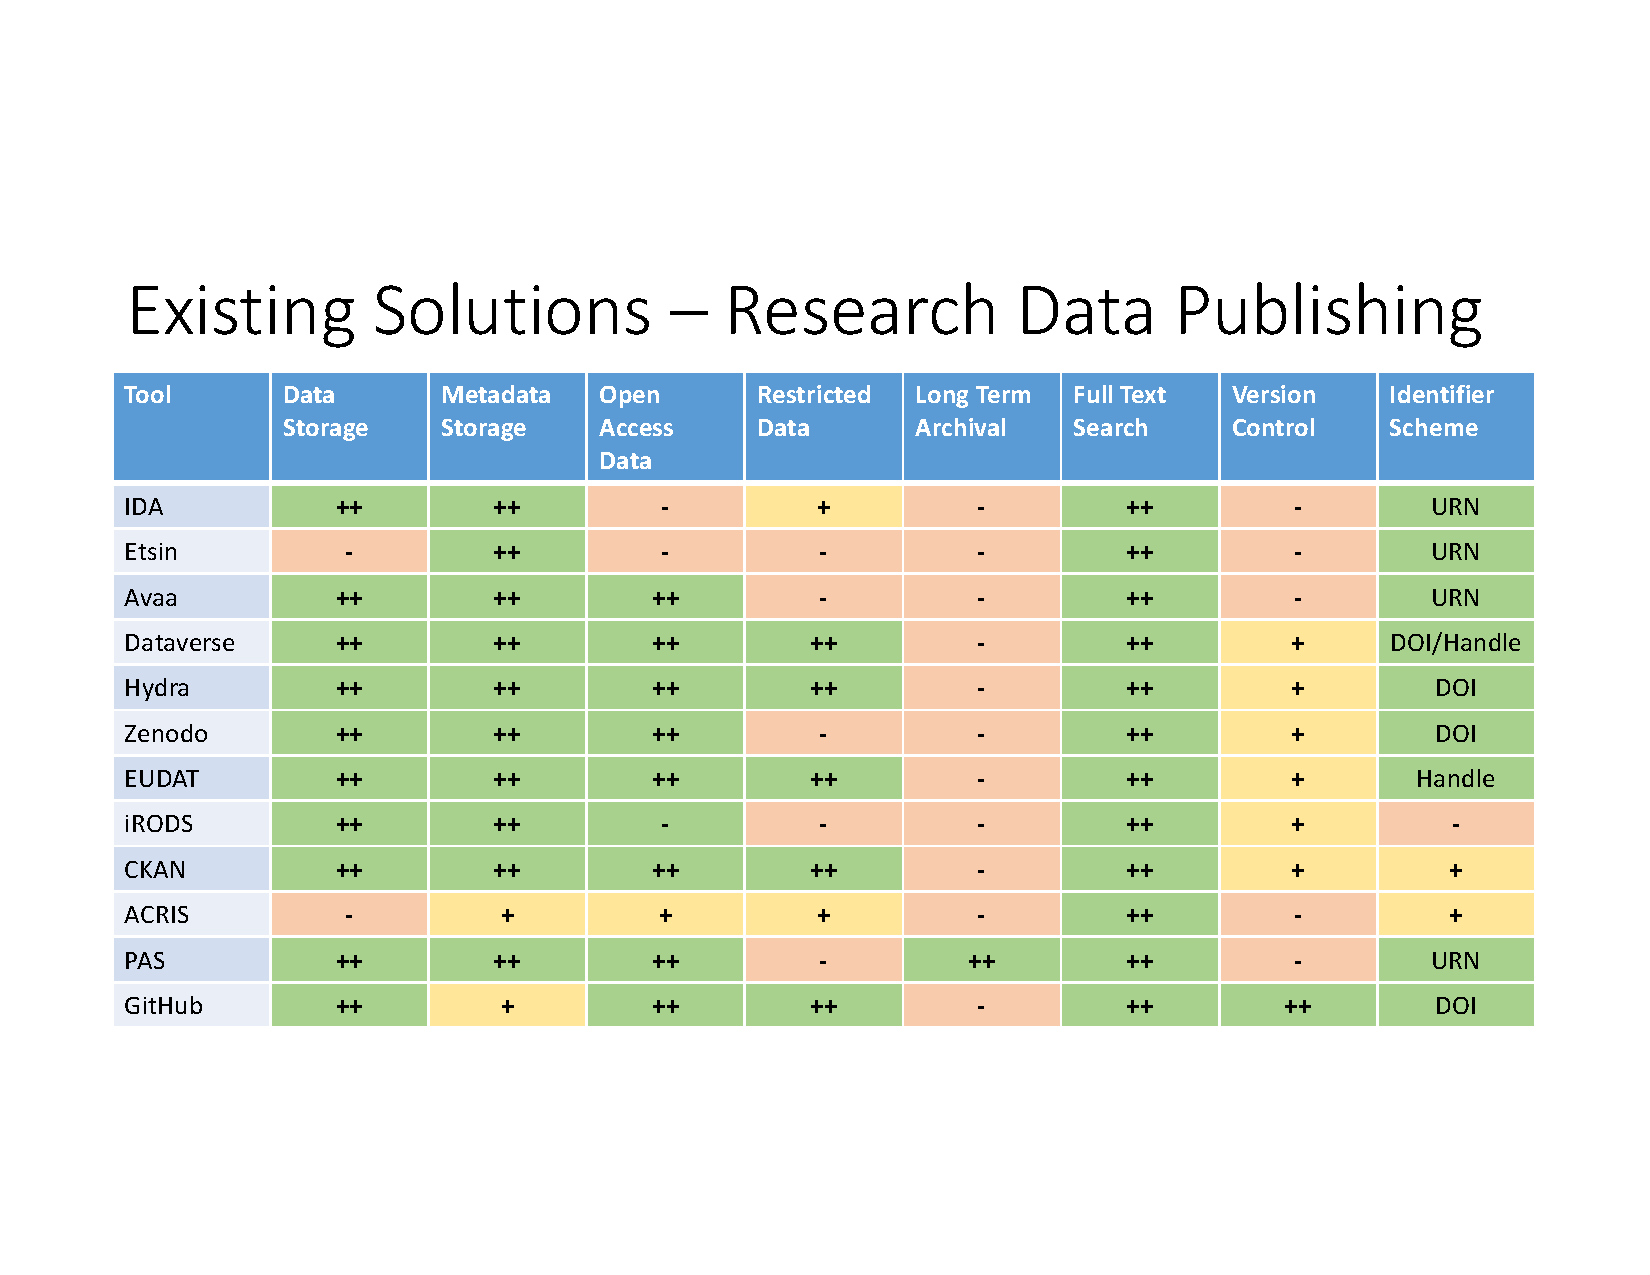
\includegraphics[width=\textwidth]{images/publishing}
    \end{centering}
    \caption{A placeholder for the latex table}
    \label{fig:solutions}
\end{sidewaysfigure}

Research data publishing is the end goal of research data management, and
Table \ref{fig:management} shows the same tools being compared in the light
of research data management during the research process.

\begin{sidewaysfigure}
    \begin{centering}
        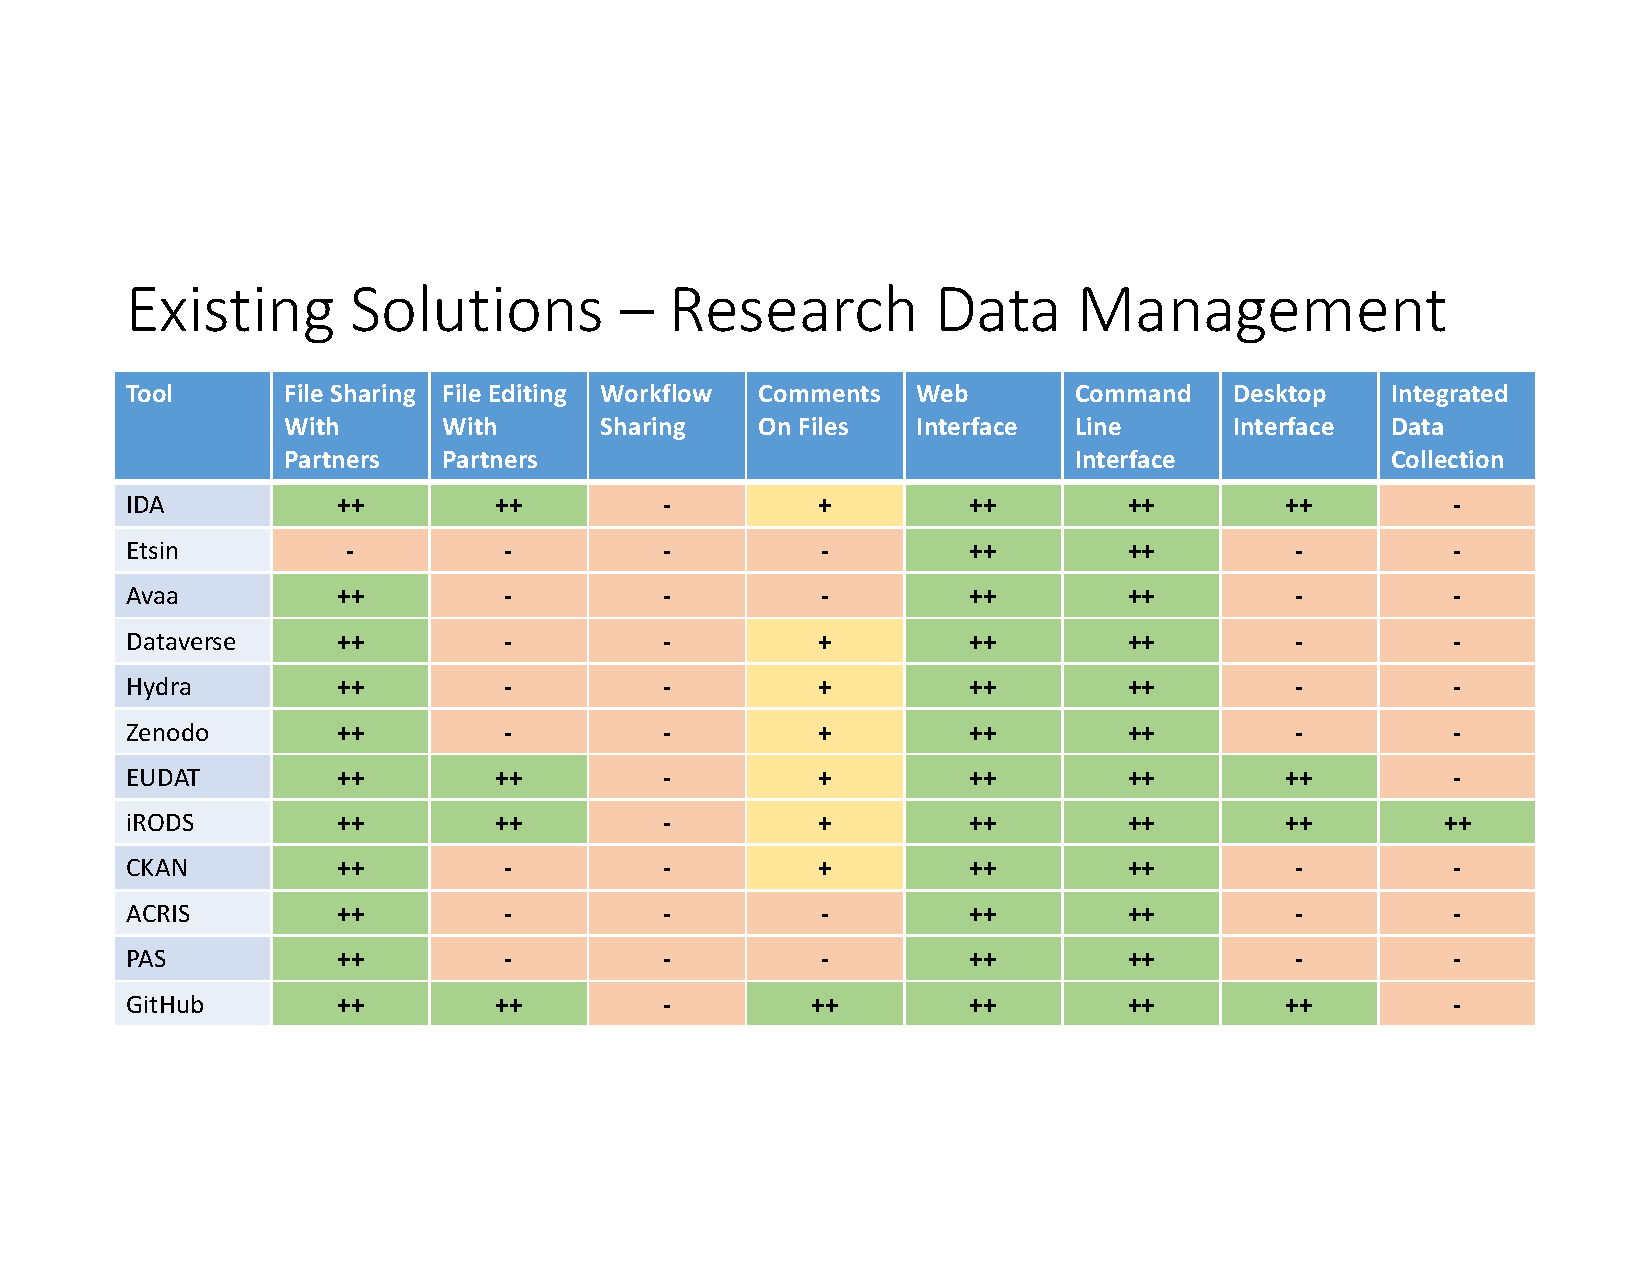
\includegraphics[width=\textwidth]{images/management}
    \end{centering}
    \caption{A placeholder for the latex table}
    \label{fig:management}
\end{sidewaysfigure}

The same tools that are suitable for research data publishing are not
necessarily right for research data management and vice versa. Technical
point solutions for both exist, but a solution that takes care of the whole
lifecycle of the data is what is needed.

This thesis also identified many aspects of a solution that could solve the
research data management and sharing problem. These requirements are split
into functional, hardware and experiental requirements and are shown below
in Tables (TODO: put tables here). The presented requirements could be used
to design a research data management and publishing solution as well as to
validate an existing solution.

(REQUIREMENT TABLES HERE)

Technical solutions alone are not enough to make research data management
and publishing a reality. The culture about open research data has to be
changed so that it's natural and rewarding for people to publish and take
good care of their research data. This requires training, commitment from
research institutions and people to advocate for the cause.
